\section{Classical learning}
Difference between Supervised unsupervised.


%%%%%%%%%%%%%%%%%%%%%%%%%%%%%%%%%%%%%%%%%%%%%%%%%%%%%%%%%

\subsection{Supervised}
Um einen Abfragepunkt zu klassifizieren, nutzt diese Methode die gespeicherten

%%%%%%%%%%%%%%%%%%%%%%%%%%%%%%%%%%%%%%%%%%%%%%%%%%%%%%%%%

\subsection{Support Vector Machine}
\subsubsection{Introduction}

Support Vector Machines (SVM) are supervised learning algorithms for classification.
They are one of the most widely used supervised learning algorithms. 
SVMs offer a high accuracy when it comes to classification.
The idea behind a SVM is to find a hyperplane that seperates classes of datapoints with a large margin. Where the margin is the smallest distance between the closest datapoint $x$ of one class and the hyperplane (therfore the name 'support vector'). Because of this feature the SVM is sometimes also called \textbf{large margin classifier}.
The so called kernel trick can be applied when non linear data has to be classified.

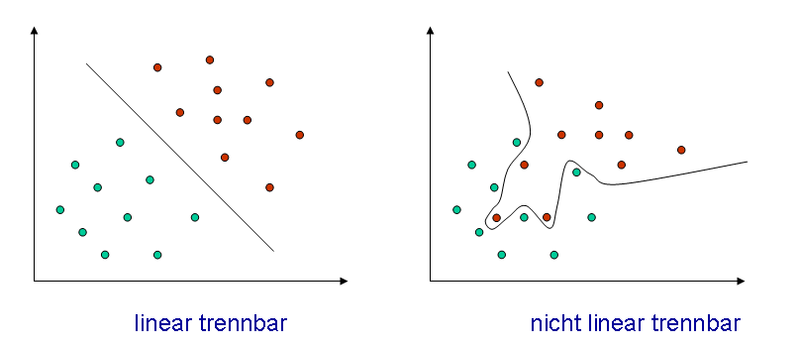
\includegraphics[scale=0.5]{Images/svm.png}


\subsubsection{Mathematics behind SVMs}
For given input data $X = \{x_{1}, ..., x_{m}\}$, with $x_{i} \in \mathbb{R}^n$ and matching result vector $Y = \{y_{1}, ..., y_{m}\}$, with $y_{i} \in \{-1, 1\}$. We want a classifier \\ $h: \mathbb{R}^{n} \rightarrow \{-1, 1\}$ such that $h(x) = $ $\begin{cases*} 1 & ,if $ w^{T} x + b  > 0$,\\ -1& ,if $w^{T} x+b < 0$.\end{cases*}$ with $w \in \mathbb{R}^{n}$ and $b \in \mathbb{R}$. We want h to be correct for most samples. This formulation leads to the following primal problem: \\
$min_{w,b,s} \frac{1}{2} w w^T + C \sum_{i = 1}^m s_{i}$, \\
s.t.: $y_i (w^T x_i + b ) \geq 1 - s_i$, $s_i \geq 0$. \\
Where $s_i$ are the so called slack variables that should denote the distance from the correct margin if a point is misclassified. \\
Intuitively we want to maximize the margin what results in minimizing $||w||^2$ including a penalty when something is misclassified.
$C$ controlls the strength of the misclassification penaly. One could view it as a inverse regularization parameter. A large C results in overfitting and a smaller C results in a "smoother" fit.\\
The dual problem to the above Primal problem is: \\
$min_{\lambda} \frac{1}{2} \lambda^T Q \lambda - e^T \lambda$ \\
s.t.: $y^T \lambda = 0$ and $0 \leq \lambda_{i} \leq C$ for all $i = 1,...,m$.
The entries of the matrix $Q \in \mathbb{R}^{m \times m}$ are given by $Q_{i, j} = y_i y_j \langle x_i, x_j \rangle$. \\
This shows that the minimization only depends on the scalar product of $x_i$ and $x_j$ and we can apply the kernel trick. Instead of the standard scalar product we can use a kernel function $K(x_i, x_j)$.

\subsubsection{In our case}
We use the python library sklearn, which can easily be installed via pip.
First we get the training data and split it into training and test data.\\
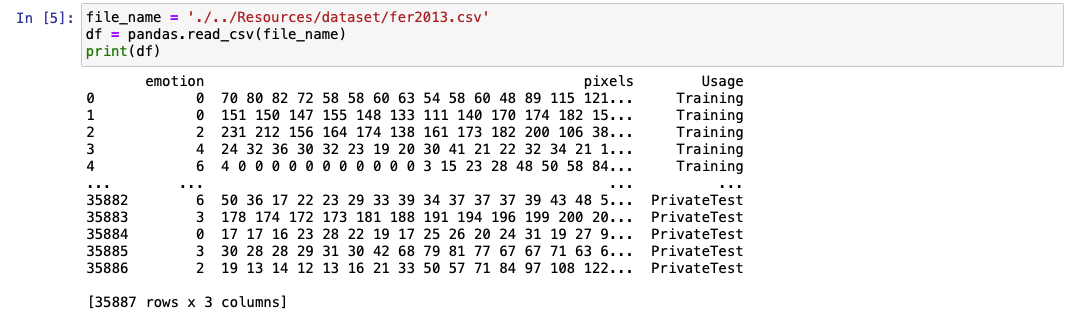
\includegraphics[scale=0.4]{Images/trainingdata.png} \\
Next we fit the model to the training data for the chosen parameters and safe it with the pickle model. \\
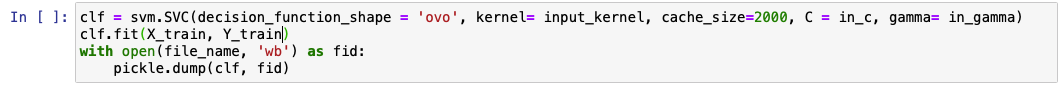
\includegraphics[scale=0.4]{Images/trainmodel.png} \\
Now the model can give a prediction on new images. \\
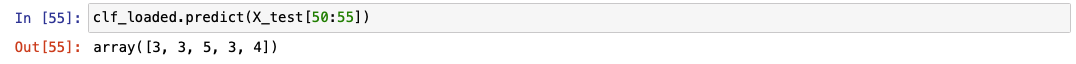
\includegraphics[scale=0.4]{Images/svm_prediction.png}



%%%%%%%%%%%%%%%%%%%%%%%%%%%%%%%%%%%%%%%%%%%%%%%%%%%%%%%%%

\subsubsection{Regression}
Like for all other subsubsections i would sugest that we structure the Algorithms like in the table at Ch.2.(\textbf{\underline{Algorithm}}, \textbf{\underline{possible application}}, etc.), but also add some links etc. Trainingsdaten und berechnet den Abstand zu den jeweiligen Merkmalen. In 
 
%%%%%%%%%%%%%%%%%%%%%%%%%%%%%%%%%%%%%%%%%%%%%%%%%%%%%%%%%

\subsubsection{Classification}
See regression
%%%%%%%%%%%%%%%%%%%%%%%%%%%%%%%%%%%%%%%%%%%%%%%%%%%%%%%%%

\subsection{Unsupervised}
See regression

%%%%%%%%%%%%%%%%%%%%%%%%%%%%%%%%%%%%%%%%%%%%%%%%%%%%%%%%%

\subsubsection{Clustering}
See regression
 
%%%%%%%%%%%%%%%%%%%%%%%%%%%%%%%%%%%%%%%%%%%%%%%%%%%%%%%%%

\subsubsection{Pattern search}
See regression
%%%%%%%%%%%%%%%%%%%%%%%%%%%%%%%%%%%%%%%%%%%%%%%%%%%%%%%%%

\subsubsection{Dimension Reduction}
See regression

%%%%%%%%%%%%%%%%%%%%%%%%%%%%%%%%%%%%%%%%%%%%%%%%%%%%%%%%%
 


\newpage